\documentclass[1p]{elsarticle_modified}
%\bibliographystyle{elsarticle-num}

%\usepackage[colorlinks]{hyperref}
%\usepackage{abbrmath_seonhwa} %\Abb, \Ascr, \Acal ,\Abf, \Afrak
\usepackage{amsfonts}
\usepackage{amssymb}
\usepackage{amsmath}
\usepackage{amsthm}
\usepackage{scalefnt}
\usepackage{amsbsy}
\usepackage{kotex}
\usepackage{caption}
\usepackage{subfig}
\usepackage{color}
\usepackage{graphicx}
\usepackage{xcolor} %% white, black, red, green, blue, cyan, magenta, yellow
\usepackage{float}
\usepackage{setspace}
\usepackage{hyperref}

\usepackage{tikz}
\usetikzlibrary{arrows}

\usepackage{multirow}
\usepackage{array} % fixed length table
\usepackage{hhline}

%%%%%%%%%%%%%%%%%%%%%
\makeatletter
\renewcommand*\env@matrix[1][\arraystretch]{%
	\edef\arraystretch{#1}%
	\hskip -\arraycolsep
	\let\@ifnextchar\new@ifnextchar
	\array{*\c@MaxMatrixCols c}}
\makeatother %https://tex.stackexchange.com/questions/14071/how-can-i-increase-the-line-spacing-in-a-matrix
%%%%%%%%%%%%%%%

\usepackage[normalem]{ulem}

\newcommand{\msout}[1]{\ifmmode\text{\sout{\ensuremath{#1}}}\else\sout{#1}\fi}
%SOURCE: \msout is \stkout macro in https://tex.stackexchange.com/questions/20609/strikeout-in-math-mode

\newcommand{\cancel}[1]{
	\ifmmode
	{\color{red}\msout{#1}}
	\else
	{\color{red}\sout{#1}}
	\fi
}

\newcommand{\add}[1]{
	{\color{blue}\uwave{#1}}
}

\newcommand{\replace}[2]{
	\ifmmode
	{\color{red}\msout{#1}}{\color{blue}\uwave{#2}}
	\else
	{\color{red}\sout{#1}}{\color{blue}\uwave{#2}}
	\fi
}

\newcommand{\Sol}{\mathcal{S}} %segment
\newcommand{\D}{D} %diagram
\newcommand{\A}{\mathcal{A}} %arc


%%%%%%%%%%%%%%%%%%%%%%%%%%%%%5 test

\def\sl{\operatorname{\textup{SL}}(2,\Cbb)}
\def\psl{\operatorname{\textup{PSL}}(2,\Cbb)}
\def\quan{\mkern 1mu \triangleright \mkern 1mu}

\theoremstyle{definition}
\newtheorem{thm}{Theorem}[section]
\newtheorem{prop}[thm]{Proposition}
\newtheorem{lem}[thm]{Lemma}
\newtheorem{ques}[thm]{Question}
\newtheorem{cor}[thm]{Corollary}
\newtheorem{defn}[thm]{Definition}
\newtheorem{exam}[thm]{Example}
\newtheorem{rmk}[thm]{Remark}
\newtheorem{alg}[thm]{Algorithm}

\newcommand{\I}{\sqrt{-1}}
\begin{document}

%\begin{frontmatter}
%
%\title{Boundary parabolic representations of knots up to 8 crossings}
%
%%% Group authors per affiliation:
%\author{Yunhi Cho} 
%\address{Department of Mathematics, University of Seoul, Seoul, Korea}
%\ead{yhcho@uos.ac.kr}
%
%
%\author{Seonhwa Kim} %\fnref{s_kim}}
%\address{Center for Geometry and Physics, Institute for Basic Science, Pohang, 37673, Korea}
%\ead{ryeona17@ibs.re.kr}
%
%\author{Hyuk Kim}
%\address{Department of Mathematical Sciences, Seoul National University, Seoul 08826, Korea}
%\ead{hyukkim@snu.ac.kr}
%
%\author{Seokbeom Yoon}
%\address{Department of Mathematical Sciences, Seoul National University, Seoul, 08826,  Korea}
%\ead{sbyoon15@snu.ac.kr}
%
%\begin{abstract}
%We find all boundary parabolic representation of knots up to 8 crossings.
%
%\end{abstract}
%\begin{keyword}
%    \MSC[2010] 57M25 
%\end{keyword}
%
%\end{frontmatter}

%\linenumbers
%\tableofcontents
%
\newcommand\colored[1]{\textcolor{white}{\rule[-0.35ex]{0.8em}{1.4ex}}\kern-0.8em\color{red} #1}%
%\newcommand\colored[1]{\textcolor{white}{ #1}\kern-2.17ex	\textcolor{white}{ #1}\kern-1.81ex	\textcolor{white}{ #1}\kern-2.15ex\color{red}#1	}

{\Large $\underline{12a_{0886}~(K12a_{0886})}$}

\setlength{\tabcolsep}{10pt}
\renewcommand{\arraystretch}{1.6}
\vspace{1cm}\begin{tabular}{m{100pt}>{\centering\arraybackslash}m{274pt}}
\multirow{5}{120pt}{
	\centering
	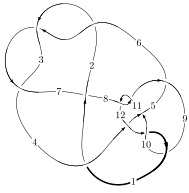
\includegraphics[width=112pt]{../../../GIT/diagram.site/Diagrams/png/1687_12a_0886.png}\\
\ \ \ A knot diagram\footnotemark}&
\allowdisplaybreaks
\textbf{Linearized knot diagam} \\
\cline{2-2}
 &
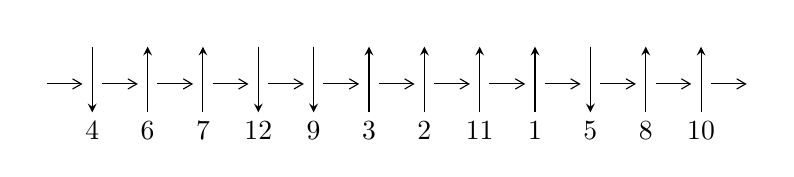
\begin{tikzpicture}[x=20pt, y=17pt]
	% nodes
	\node (C0) at (0, 0) {};
	\node (C1) at (1, 0) {};
	\node (C1U) at (1, +1) {};
	\node (C1D) at (1, -1) {4};

	\node (C2) at (2, 0) {};
	\node (C2U) at (2, +1) {};
	\node (C2D) at (2, -1) {6};

	\node (C3) at (3, 0) {};
	\node (C3U) at (3, +1) {};
	\node (C3D) at (3, -1) {7};

	\node (C4) at (4, 0) {};
	\node (C4U) at (4, +1) {};
	\node (C4D) at (4, -1) {12};

	\node (C5) at (5, 0) {};
	\node (C5U) at (5, +1) {};
	\node (C5D) at (5, -1) {9};

	\node (C6) at (6, 0) {};
	\node (C6U) at (6, +1) {};
	\node (C6D) at (6, -1) {3};

	\node (C7) at (7, 0) {};
	\node (C7U) at (7, +1) {};
	\node (C7D) at (7, -1) {2};

	\node (C8) at (8, 0) {};
	\node (C8U) at (8, +1) {};
	\node (C8D) at (8, -1) {11};

	\node (C9) at (9, 0) {};
	\node (C9U) at (9, +1) {};
	\node (C9D) at (9, -1) {1};

	\node (C10) at (10, 0) {};
	\node (C10U) at (10, +1) {};
	\node (C10D) at (10, -1) {5};

	\node (C11) at (11, 0) {};
	\node (C11U) at (11, +1) {};
	\node (C11D) at (11, -1) {8};

	\node (C12) at (12, 0) {};
	\node (C12U) at (12, +1) {};
	\node (C12D) at (12, -1) {10};
	\node (C13) at (13, 0) {};

	% arrows
	\draw[->,>={angle 60}]
	(C0) edge (C1) (C1) edge (C2) (C2) edge (C3) (C3) edge (C4) (C4) edge (C5) (C5) edge (C6) (C6) edge (C7) (C7) edge (C8) (C8) edge (C9) (C9) edge (C10) (C10) edge (C11) (C11) edge (C12) (C12) edge (C13) ;	\draw[->,>=stealth]
	(C1U) edge (C1D) (C2D) edge (C2U) (C3D) edge (C3U) (C4U) edge (C4D) (C5U) edge (C5D) (C6D) edge (C6U) (C7D) edge (C7U) (C8D) edge (C8U) (C9D) edge (C9U) (C10U) edge (C10D) (C11D) edge (C11U) (C12D) edge (C12U) ;
	\end{tikzpicture} \\
\hhline{~~} \\& 
\textbf{Solving Sequence} \\ \cline{2-2} 
 &
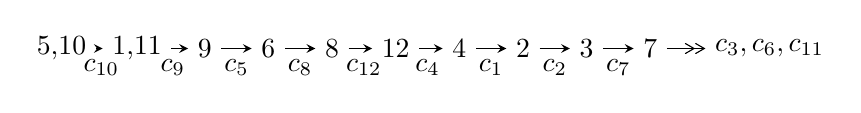
\begin{tikzpicture}[x=23pt, y=7pt]
	% node
	\node (A0) at (-1/8, 0) {5,10};
	\node (A1) at (17/16, 0) {1,11};
	\node (A2) at (17/8, 0) {9};
	\node (A3) at (25/8, 0) {6};
	\node (A4) at (33/8, 0) {8};
	\node (A5) at (41/8, 0) {12};
	\node (A6) at (49/8, 0) {4};
	\node (A7) at (57/8, 0) {2};
	\node (A8) at (65/8, 0) {3};
	\node (A9) at (73/8, 0) {7};
	\node (C1) at (1/2, -1) {$c_{10}$};
	\node (C2) at (13/8, -1) {$c_{9}$};
	\node (C3) at (21/8, -1) {$c_{5}$};
	\node (C4) at (29/8, -1) {$c_{8}$};
	\node (C5) at (37/8, -1) {$c_{12}$};
	\node (C6) at (45/8, -1) {$c_{4}$};
	\node (C7) at (53/8, -1) {$c_{1}$};
	\node (C8) at (61/8, -1) {$c_{2}$};
	\node (C9) at (69/8, -1) {$c_{7}$};
	\node (A10) at (11, 0) {$c_{3},c_{6},c_{11}$};

	% edge
	\draw[->,>=stealth]	
	(A0) edge (A1) (A1) edge (A2) (A2) edge (A3) (A3) edge (A4) (A4) edge (A5) (A5) edge (A6) (A6) edge (A7) (A7) edge (A8) (A8) edge (A9) ;
	\draw[->>,>={angle 60}]	
	(A9) edge (A10);
\end{tikzpicture} \\ 

\end{tabular} \\

\footnotetext{
The image of knot diagram is generated by the software ``\textbf{Draw programme}" developed by Andrew Bartholomew(\url{http://www.layer8.co.uk/maths/draw/index.htm\#Running-draw}), where we modified some parts for our purpose(\url{https://github.com/CATsTAILs/LinksPainter}).
}\phantom \\ \newline 
\centering \textbf{Ideals for irreducible components\footnotemark of $X_{\text{par}}$} 
 
\begin{align*}
I^u_{1}&=\langle 
5.07214\times10^{121} u^{41}-1.29009\times10^{122} u^{40}+\cdots+1.79683\times10^{124} b-2.09627\times10^{125},\\
\phantom{I^u_{1}}&\phantom{= \langle  }1.21110\times10^{125} u^{41}-3.08153\times10^{125} u^{40}+\cdots+3.67991\times10^{127} a-5.44579\times10^{128},\\
\phantom{I^u_{1}}&\phantom{= \langle  }u^{42}-3 u^{41}+\cdots-7680 u+2048\rangle \\
I^u_{2}&=\langle 
- u^2 a+b-1,\;-4 u^{32} a-6 u^{31} a+\cdots+a+8,\;u^{33}+2 u^{32}+\cdots-2 u-1\rangle \\
I^u_{3}&=\langle 
b- a-1,\;a^2+a+2,\;u-1\rangle \\
I^u_{4}&=\langle 
b- u,\;a-1,\;u^2+1\rangle \\
\\
I^v_{1}&=\langle 
a,\;b+1,\;32 v^5+16 v^4+16 v^3+4 v^2+2 v+1\rangle \\
\end{align*}
\raggedright * 5 irreducible components of $\dim_{\mathbb{C}}=0$, with total 117 representations.\\
\footnotetext{All coefficients of polynomials are rational numbers. But the coefficients are sometimes approximated in decimal forms when there is not enough margin.}
\newpage
\renewcommand{\arraystretch}{1}
\centering \section*{I. $I^u_{1}= \langle 5.07\times10^{121} u^{41}-1.29\times10^{122} u^{40}+\cdots+1.80\times10^{124} b-2.10\times10^{125},\;1.21\times10^{125} u^{41}-3.08\times10^{125} u^{40}+\cdots+3.68\times10^{127} a-5.45\times10^{128},\;u^{42}-3 u^{41}+\cdots-7680 u+2048 \rangle$}
\flushleft \textbf{(i) Arc colorings}\\
\begin{tabular}{m{7pt} m{180pt} m{7pt} m{180pt} }
\flushright $a_{5}=$&$\begin{pmatrix}0\\u\end{pmatrix}$ \\
\flushright $a_{10}=$&$\begin{pmatrix}1\\0\end{pmatrix}$ \\
\flushright $a_{1}=$&$\begin{pmatrix}-0.00329111 u^{41}+0.00837392 u^{40}+\cdots-21.9426 u+14.7987\\-0.00282282 u^{41}+0.00717978 u^{40}+\cdots-18.7314 u+11.6665\end{pmatrix}$ \\
\flushright $a_{11}=$&$\begin{pmatrix}1\\u^2\end{pmatrix}$ \\
\flushright $a_{9}=$&$\begin{pmatrix}-0.000468286 u^{41}+0.00119414 u^{40}+\cdots-3.21121 u+3.13219\\0.00274209 u^{41}-0.00695770 u^{40}+\cdots+18.0721 u-11.2349\end{pmatrix}$ \\
\flushright $a_{6}=$&$\begin{pmatrix}0.000392195 u^{41}-0.00107102 u^{40}+\cdots+1.79714 u-2.03513\\-0.00149906 u^{41}+0.00367622 u^{40}+\cdots-10.2811 u+6.35866\end{pmatrix}$ \\
\flushright $a_{8}=$&$\begin{pmatrix}-0.00329111 u^{41}+0.00837392 u^{40}+\cdots-21.9426 u+14.7987\\0.00208209 u^{41}-0.00535290 u^{40}+\cdots+13.9562 u-8.59570\end{pmatrix}$ \\
\flushright $a_{12}=$&$\begin{pmatrix}-0.000468286 u^{41}+0.00119414 u^{40}+\cdots-3.21121 u+3.13219\\-0.00282282 u^{41}+0.00717978 u^{40}+\cdots-18.7314 u+11.6665\end{pmatrix}$ \\
\flushright $a_{4}=$&$\begin{pmatrix}-0.000392195 u^{41}+0.00107102 u^{40}+\cdots-1.79714 u+2.03513\\-0.00147930 u^{41}+0.00368763 u^{40}+\cdots-10.2886 u+6.57486\end{pmatrix}$ \\
\flushright $a_{2}=$&$\begin{pmatrix}-0.00305058 u^{41}+0.00802983 u^{40}+\cdots-20.7780 u+15.1603\\-0.00409737 u^{41}+0.0103081 u^{40}+\cdots-27.3367 u+16.8188\end{pmatrix}$ \\
\flushright $a_{3}=$&$\begin{pmatrix}-0.00676311 u^{41}+0.0172674 u^{40}+\cdots-46.9837 u+30.8098\\-0.00457559 u^{41}+0.0113420 u^{40}+\cdots-32.3525 u+17.7346\end{pmatrix}$ \\
\flushright $a_{7}=$&$\begin{pmatrix}-0.00676311 u^{41}+0.0172674 u^{40}+\cdots-46.9837 u+30.8098\\0.00331935 u^{41}-0.00806990 u^{40}+\cdots+22.9950 u-11.5457\end{pmatrix}$\\&\end{tabular}
\flushleft \textbf{(ii) Obstruction class $= -1$}\\~\\
\flushleft \textbf{(iii) Cusp Shapes $= -0.0230966 u^{41}+0.0573171 u^{40}+\cdots-173.318 u+88.0642$}\\~\\
\newpage\renewcommand{\arraystretch}{1}
\flushleft \textbf{(iv) u-Polynomials at the component}\newline \\
\begin{tabular}{m{50pt}|m{274pt}}
Crossings & \hspace{64pt}u-Polynomials at each crossing \\
\hline $$\begin{aligned}c_{1}\end{aligned}$$&$\begin{aligned}
&u^{42}-10 u^{41}+\cdots-11111 u+1504
\end{aligned}$\\
\hline $$\begin{aligned}c_{2},c_{3},c_{6}\end{aligned}$$&$\begin{aligned}
&u^{42}-2 u^{41}+\cdots+7 u-4
\end{aligned}$\\
\hline $$\begin{aligned}c_{4},c_{5}\end{aligned}$$&$\begin{aligned}
&32(32 u^{42}+48 u^{41}+\cdots+20 u^2+2)
\end{aligned}$\\
\hline $$\begin{aligned}c_{7}\end{aligned}$$&$\begin{aligned}
&u^{42}-2 u^{40}+\cdots+1136 u-448
\end{aligned}$\\
\hline $$\begin{aligned}c_{8},c_{9},c_{11}\\c_{12}\end{aligned}$$&$\begin{aligned}
&u^{42}-5 u^{41}+\cdots- u-1
\end{aligned}$\\
\hline $$\begin{aligned}c_{10}\end{aligned}$$&$\begin{aligned}
&u^{42}-3 u^{41}+\cdots-7680 u+2048
\end{aligned}$\\
\hline
\end{tabular}\\~\\
\newpage\renewcommand{\arraystretch}{1}
\flushleft \textbf{(v) Riley Polynomials at the component}\newline \\
\begin{tabular}{m{50pt}|m{274pt}}
Crossings & \hspace{64pt}Riley Polynomials at each crossing \\
\hline $$\begin{aligned}c_{1}\end{aligned}$$&$\begin{aligned}
&y^{42}+14 y^{41}+\cdots+62115215 y+2262016
\end{aligned}$\\
\hline $$\begin{aligned}c_{2},c_{3},c_{6}\end{aligned}$$&$\begin{aligned}
&y^{42}-38 y^{41}+\cdots- y+16
\end{aligned}$\\
\hline $$\begin{aligned}c_{4},c_{5}\end{aligned}$$&$\begin{aligned}
&1024(1024 y^{42}-1280 y^{41}+\cdots+80 y+4)
\end{aligned}$\\
\hline $$\begin{aligned}c_{7}\end{aligned}$$&$\begin{aligned}
&y^{42}-4 y^{41}+\cdots-2874624 y+200704
\end{aligned}$\\
\hline $$\begin{aligned}c_{8},c_{9},c_{11}\\c_{12}\end{aligned}$$&$\begin{aligned}
&y^{42}+17 y^{41}+\cdots+9 y+1
\end{aligned}$\\
\hline $$\begin{aligned}c_{10}\end{aligned}$$&$\begin{aligned}
&y^{42}-9 y^{41}+\cdots-69468160 y+4194304
\end{aligned}$\\
\hline
\end{tabular}\\~\\
\newpage\flushleft \textbf{(vi) Complex Volumes and Cusp Shapes}
$$\begin{array}{c|c|c}  
\text{Solutions to }I^u_{1}& \I (\text{vol} + \sqrt{-1}CS) & \text{Cusp shape}\\
 \hline 
\begin{aligned}
u &= -0.314188 + 1.053170 I \\
a &= \phantom{-}0.027002 + 0.483467 I \\
b &= -0.594138 + 0.750449 I\end{aligned}
 & \phantom{-}5.98291 - 1.19095 I & \phantom{-}10.40868 + 3.12372 I \\ \hline\begin{aligned}
u &= -0.314188 - 1.053170 I \\
a &= \phantom{-}0.027002 - 0.483467 I \\
b &= -0.594138 - 0.750449 I\end{aligned}
 & \phantom{-}5.98291 + 1.19095 I & \phantom{-}10.40868 - 3.12372 I \\ \hline\begin{aligned}
u &= \phantom{-}0.820994 + 0.197858 I \\
a &= \phantom{-}0.95965 + 1.29956 I \\
b &= \phantom{-}0.291149 + 0.470080 I\end{aligned}
 & \phantom{-}6.19589 - 3.49276 I & \phantom{-}6.51052 + 0.13763 I \\ \hline\begin{aligned}
u &= \phantom{-}0.820994 - 0.197858 I \\
a &= \phantom{-}0.95965 - 1.29956 I \\
b &= \phantom{-}0.291149 - 0.470080 I\end{aligned}
 & \phantom{-}6.19589 + 3.49276 I & \phantom{-}6.51052 - 0.13763 I \\ \hline\begin{aligned}
u &= -0.577314 + 0.526253 I \\
a &= -0.108552 + 0.213642 I \\
b &= -1.121680 + 0.508475 I\end{aligned}
 & \phantom{-}8.12984 - 3.40777 I & \phantom{-}9.67454 - 1.62361 I \\ \hline\begin{aligned}
u &= -0.577314 - 0.526253 I \\
a &= -0.108552 - 0.213642 I \\
b &= -1.121680 - 0.508475 I\end{aligned}
 & \phantom{-}8.12984 + 3.40777 I & \phantom{-}9.67454 + 1.62361 I \\ \hline\begin{aligned}
u &= -0.991104 + 0.788632 I \\
a &= \phantom{-}0.430066 - 0.979780 I \\
b &= \phantom{-}0.048227 - 0.652088 I\end{aligned}
 & \phantom{-}0.103272 + 0.890316 I & \phantom{-}7.21863 - 1.89711 I \\ \hline\begin{aligned}
u &= -0.991104 - 0.788632 I \\
a &= \phantom{-}0.430066 + 0.979780 I \\
b &= \phantom{-}0.048227 + 0.652088 I\end{aligned}
 & \phantom{-}0.103272 - 0.890316 I & \phantom{-}7.21863 + 1.89711 I \\ \hline\begin{aligned}
u &= \phantom{-}0.650573 + 0.315344 I \\
a &= -0.150923 - 0.123948 I \\
b &= -1.306350 - 0.336680 I\end{aligned}
 & \phantom{-}7.29715 - 5.25882 I & \phantom{-}4.50219 + 8.83294 I \\ \hline\begin{aligned}
u &= \phantom{-}0.650573 - 0.315344 I \\
a &= -0.150923 + 0.123948 I \\
b &= -1.306350 + 0.336680 I\end{aligned}
 & \phantom{-}7.29715 + 5.25882 I & \phantom{-}4.50219 - 8.83294 I\\
 \hline 
 \end{array}$$\newpage$$\begin{array}{c|c|c}  
\text{Solutions to }I^u_{1}& \I (\text{vol} + \sqrt{-1}CS) & \text{Cusp shape}\\
 \hline 
\begin{aligned}
u &= -0.375562 + 0.527351 I \\
a &= \phantom{-}0.695747 - 0.521764 I \\
b &= -0.077418 - 0.331511 I\end{aligned}
 & \phantom{-}0.199443 + 0.975184 I & \phantom{-}4.03278 - 6.08768 I \\ \hline\begin{aligned}
u &= -0.375562 - 0.527351 I \\
a &= \phantom{-}0.695747 + 0.521764 I \\
b &= -0.077418 + 0.331511 I\end{aligned}
 & \phantom{-}0.199443 - 0.975184 I & \phantom{-}4.03278 + 6.08768 I \\ \hline\begin{aligned}
u &= -1.354830 + 0.085427 I \\
a &= \phantom{-}0.20811 + 1.54932 I \\
b &= \phantom{-}0.374024 + 0.802773 I\end{aligned}
 & \phantom{-}5.97161 + 6.59731 I & \phantom{-}7.43283 - 8.44870 I \\ \hline\begin{aligned}
u &= -1.354830 - 0.085427 I \\
a &= \phantom{-}0.20811 - 1.54932 I \\
b &= \phantom{-}0.374024 - 0.802773 I\end{aligned}
 & \phantom{-}5.97161 - 6.59731 I & \phantom{-}7.43283 + 8.44870 I \\ \hline\begin{aligned}
u &= -0.570711 + 0.284785 I \\
a &= -0.119513 + 0.107746 I \\
b &= -1.237960 + 0.273860 I\end{aligned}
 & \phantom{-}1.86047 + 2.11675 I & -0.90328 - 11.17612 I \\ \hline\begin{aligned}
u &= -0.570711 - 0.284785 I \\
a &= -0.119513 - 0.107746 I \\
b &= -1.237960 - 0.273860 I\end{aligned}
 & \phantom{-}1.86047 - 2.11675 I & -0.90328 + 11.17612 I \\ \hline\begin{aligned}
u &= \phantom{-}0.442682 + 0.457127 I \\
a &= -0.050983 - 0.171060 I \\
b &= -1.041130 - 0.367914 I\end{aligned}
 & \phantom{-}2.47985 + 1.01844 I & \phantom{-}7.66650 + 3.92369 I \\ \hline\begin{aligned}
u &= \phantom{-}0.442682 - 0.457127 I \\
a &= -0.050983 + 0.171060 I \\
b &= -1.041130 + 0.367914 I\end{aligned}
 & \phantom{-}2.47985 - 1.01844 I & \phantom{-}7.66650 - 3.92369 I \\ \hline\begin{aligned}
u &= \phantom{-}0.522304\phantom{ +0.000000I} \\
a &= -0.110575\phantom{ +0.000000I} \\
b &= -1.24864\phantom{ +0.000000I}\end{aligned}
 & \phantom{-}3.67439\phantom{ +0.000000I} & -7.95490\phantom{ +0.000000I} \\ \hline\begin{aligned}
u &= \phantom{-}1.54341 + 0.23309 I \\
a &= \phantom{-}0.243734 + 1.309960 I \\
b &= \phantom{-}0.237641 + 0.802950 I\end{aligned}
 & -0.35149 + 3.39390 I & \phantom{-0.000000 } 0. - 8.80504 I\\
 \hline 
 \end{array}$$\newpage$$\begin{array}{c|c|c}  
\text{Solutions to }I^u_{1}& \I (\text{vol} + \sqrt{-1}CS) & \text{Cusp shape}\\
 \hline 
\begin{aligned}
u &= \phantom{-}1.54341 - 0.23309 I \\
a &= \phantom{-}0.243734 - 1.309960 I \\
b &= \phantom{-}0.237641 - 0.802950 I\end{aligned}
 & -0.35149 - 3.39390 I & \phantom{-0.000000 -}0. + 8.80504 I \\ \hline\begin{aligned}
u &= \phantom{-}0.433072\phantom{ +0.000000I} \\
a &= \phantom{-}1.51195\phantom{ +0.000000I} \\
b &= \phantom{-}0.203807\phantom{ +0.000000I}\end{aligned}
 & \phantom{-}2.70015\phantom{ +0.000000I} & \phantom{-}1.03960\phantom{ +0.000000I} \\ \hline\begin{aligned}
u &= -1.32959 + 0.84020 I \\
a &= -0.48736 + 1.45749 I \\
b &= \phantom{-}0.570490 + 1.221150 I\end{aligned}
 & \phantom{-}2.85618 + 8.34848 I & \phantom{-0.000000 } 0 \\ \hline\begin{aligned}
u &= -1.32959 - 0.84020 I \\
a &= -0.48736 - 1.45749 I \\
b &= \phantom{-}0.570490 - 1.221150 I\end{aligned}
 & \phantom{-}2.85618 - 8.34848 I & \phantom{-0.000000 } 0 \\ \hline\begin{aligned}
u &= \phantom{-}1.29599 + 0.93912 I \\
a &= -0.58004 - 1.38071 I \\
b &= \phantom{-}0.59672 - 1.32586 I\end{aligned}
 & \phantom{-}0.1604 - 18.2186 I & \phantom{-0.000000 -}0. + 9.92364 I \\ \hline\begin{aligned}
u &= \phantom{-}1.29599 - 0.93912 I \\
a &= -0.58004 + 1.38071 I \\
b &= \phantom{-}0.59672 + 1.32586 I\end{aligned}
 & \phantom{-}0.1604 + 18.2186 I & \phantom{-0.000000 } 0. - 9.92364 I \\ \hline\begin{aligned}
u &= -1.32065 + 0.93583 I \\
a &= -0.55241 + 1.37129 I \\
b &= \phantom{-}0.56978 + 1.31805 I\end{aligned}
 & -5.4682 + 14.4315 I & \phantom{-0.000000 } 0 \\ \hline\begin{aligned}
u &= -1.32065 - 0.93583 I \\
a &= -0.55241 - 1.37129 I \\
b &= \phantom{-}0.56978 - 1.31805 I\end{aligned}
 & -5.4682 - 14.4315 I & \phantom{-0.000000 } 0 \\ \hline\begin{aligned}
u &= \phantom{-}1.35470 + 0.90995 I \\
a &= -0.50581 - 1.37917 I \\
b &= \phantom{-}0.539500 - 1.285140 I\end{aligned}
 & -4.16980 - 10.14610 I & \phantom{-0.000000 } 0 \\ \hline\begin{aligned}
u &= \phantom{-}1.35470 - 0.90995 I \\
a &= -0.50581 + 1.37917 I \\
b &= \phantom{-}0.539500 + 1.285140 I\end{aligned}
 & -4.16980 + 10.14610 I & \phantom{-0.000000 } 0\\
 \hline 
 \end{array}$$\newpage$$\begin{array}{c|c|c}  
\text{Solutions to }I^u_{1}& \I (\text{vol} + \sqrt{-1}CS) & \text{Cusp shape}\\
 \hline 
\begin{aligned}
u &= \phantom{-}0.60722 + 1.63895 I \\
a &= -0.090576 - 0.705861 I \\
b &= -0.372413 - 1.065220 I\end{aligned}
 & \phantom{-}2.41336 + 9.70431 I & \phantom{-0.000000 } 0 \\ \hline\begin{aligned}
u &= \phantom{-}0.60722 - 1.63895 I \\
a &= -0.090576 + 0.705861 I \\
b &= -0.372413 + 1.065220 I\end{aligned}
 & \phantom{-}2.41336 - 9.70431 I & \phantom{-0.000000 } 0 \\ \hline\begin{aligned}
u &= \phantom{-}1.47227 + 0.94822 I \\
a &= -0.421850 - 1.297470 I \\
b &= \phantom{-}0.426915 - 1.286100 I\end{aligned}
 & -5.57375 - 10.06480 I & \phantom{-0.000000 } 0 \\ \hline\begin{aligned}
u &= \phantom{-}1.47227 - 0.94822 I \\
a &= -0.421850 + 1.297470 I \\
b &= \phantom{-}0.426915 + 1.286100 I\end{aligned}
 & -5.57375 + 10.06480 I & \phantom{-0.000000 } 0 \\ \hline\begin{aligned}
u &= -1.57270 + 0.94944 I \\
a &= -0.352961 + 1.267110 I \\
b &= \phantom{-}0.360707 + 1.251940 I\end{aligned}
 & -8.85361 + 5.99722 I & \phantom{-0.000000 } 0 \\ \hline\begin{aligned}
u &= -1.57270 - 0.94944 I \\
a &= -0.352961 - 1.267110 I \\
b &= \phantom{-}0.360707 - 1.251940 I\end{aligned}
 & -8.85361 - 5.99722 I & \phantom{-0.000000 } 0 \\ \hline\begin{aligned}
u &= -0.47063 + 1.78264 I \\
a &= -0.047981 + 0.738048 I \\
b &= -0.312174 + 1.017260 I\end{aligned}
 & -2.89576 - 5.73091 I & \phantom{-0.000000 } 0 \\ \hline\begin{aligned}
u &= -0.47063 - 1.78264 I \\
a &= -0.047981 - 0.738048 I \\
b &= -0.312174 - 1.017260 I\end{aligned}
 & -2.89576 + 5.73091 I & \phantom{-0.000000 } 0 \\ \hline\begin{aligned}
u &= \phantom{-}0.00561 + 1.91712 I \\
a &= \phantom{-}0.046167 - 0.779412 I \\
b &= -0.229375 - 0.915905 I\end{aligned}
 & -0.81742 + 1.38862 I & \phantom{-0.000000 } 0 \\ \hline\begin{aligned}
u &= \phantom{-}0.00561 - 1.91712 I \\
a &= \phantom{-}0.046167 + 0.779412 I \\
b &= -0.229375 + 0.915905 I\end{aligned}
 & -0.81742 - 1.38862 I & \phantom{-0.000000 } 0\\
 \hline 
 \end{array}$$\newpage$$\begin{array}{c|c|c}  
\text{Solutions to }I^u_{1}& \I (\text{vol} + \sqrt{-1}CS) & \text{Cusp shape}\\
 \hline 
\begin{aligned}
u &= \phantom{-}1.70614 + 0.93966 I \\
a &= -0.279714 - 1.240500 I \\
b &= \phantom{-}0.299896 - 1.205740 I\end{aligned}
 & -4.72570 - 1.89699 I & \phantom{-0.000000 } 0 \\ \hline\begin{aligned}
u &= \phantom{-}1.70614 - 0.93966 I \\
a &= -0.279714 + 1.240500 I \\
b &= \phantom{-}0.299896 + 1.205740 I\end{aligned}
 & -4.72570 + 1.89699 I & \phantom{-0.000000 } 0\\
 \hline 
 \end{array}$$\newpage\newpage\renewcommand{\arraystretch}{1}
\centering \section*{II. $I^u_{2}= \langle - u^2 a+b-1,\;-4 u^{32} a-6 u^{31} a+\cdots+a+8,\;u^{33}+2 u^{32}+\cdots-2 u-1 \rangle$}
\flushleft \textbf{(i) Arc colorings}\\
\begin{tabular}{m{7pt} m{180pt} m{7pt} m{180pt} }
\flushright $a_{5}=$&$\begin{pmatrix}0\\u\end{pmatrix}$ \\
\flushright $a_{10}=$&$\begin{pmatrix}1\\0\end{pmatrix}$ \\
\flushright $a_{1}=$&$\begin{pmatrix}a\\u^2 a+1\end{pmatrix}$ \\
\flushright $a_{11}=$&$\begin{pmatrix}1\\u^2\end{pmatrix}$ \\
\flushright $a_{9}=$&$\begin{pmatrix}4 u^{32}+6 u^{31}+\cdots- a-2 u\\u^4 a- u^4+u^2-1\end{pmatrix}$ \\
\flushright $a_{6}=$&$\begin{pmatrix}-2 u^{32} a+u^{32}+\cdots+4 a-4\\-2 u^{32}-4 u^{31}+\cdots+9 u+4\end{pmatrix}$ \\
\flushright $a_{8}=$&$\begin{pmatrix}4 u^{32}+6 u^{31}+\cdots- a-1\\-1\end{pmatrix}$ \\
\flushright $a_{12}=$&$\begin{pmatrix}- u^2 a+a-1\\u^2 a+1\end{pmatrix}$ \\
\flushright $a_{4}=$&$\begin{pmatrix}-2 u^{32} a+3 u^{32}+\cdots+4 a-8\\-2 u^{32}-4 u^{31}+\cdots+9 u+4\end{pmatrix}$ \\
\flushright $a_{2}=$&$\begin{pmatrix}-4 u^{32}-6 u^{31}+\cdots+3 a-7\\- u^{12} a+u^{12}+\cdots-7 u^2+3\end{pmatrix}$ \\
\flushright $a_{3}=$&$\begin{pmatrix}u^{24} a-5 u^{22} a+\cdots+a-8\\u^{26} a-4 u^{24} a+\cdots-6 u^2+1\end{pmatrix}$ \\
\flushright $a_{7}=$&$\begin{pmatrix}4 u^{32}+6 u^{31}+\cdots- a+3\\u^{24} a- u^{24}+\cdots+6 u^2-1\end{pmatrix}$\\&\end{tabular}
\flushleft \textbf{(ii) Obstruction class $= -1$}\\~\\
\flushleft \textbf{(iii) Cusp Shapes $= 4 u^{32}-20 u^{30}-4 u^{29}+72 u^{28}+16 u^{27}-180 u^{26}-56 u^{25}+360 u^{24}+128 u^{23}-580 u^{22}-248 u^{21}+772 u^{20}+384 u^{19}-848 u^{18}-500 u^{17}+760 u^{16}+548 u^{15}-532 u^{14}-496 u^{13}+264 u^{12}+372 u^{11}-52 u^{10}-220 u^9-48 u^8+92 u^7+56 u^6-24 u^5-28 u^4-4 u^3+4 u^2+6$}\\~\\
\newpage\renewcommand{\arraystretch}{1}
\flushleft \textbf{(iv) u-Polynomials at the component}\newline \\
\begin{tabular}{m{50pt}|m{274pt}}
Crossings & \hspace{64pt}u-Polynomials at each crossing \\
\hline $$\begin{aligned}c_{1}\end{aligned}$$&$\begin{aligned}
&(u^{33}-6 u^{32}+\cdots+128 u-23)^{2}
\end{aligned}$\\
\hline $$\begin{aligned}c_{2},c_{3},c_{6}\end{aligned}$$&$\begin{aligned}
&(u^{33}-2 u^{32}+\cdots+u^2+1)^{2}
\end{aligned}$\\
\hline $$\begin{aligned}c_{4},c_{5}\end{aligned}$$&$\begin{aligned}
&u^{66}- u^{65}+\cdots-115818 u+36557
\end{aligned}$\\
\hline $$\begin{aligned}c_{7}\end{aligned}$$&$\begin{aligned}
&(u^{33}+3 u^{32}+\cdots+32 u+7)^{2}
\end{aligned}$\\
\hline $$\begin{aligned}c_{8},c_{9},c_{11}\\c_{12}\end{aligned}$$&$\begin{aligned}
&u^{66}+10 u^{65}+\cdots+4 u+1
\end{aligned}$\\
\hline $$\begin{aligned}c_{10}\end{aligned}$$&$\begin{aligned}
&(u^{33}+2 u^{32}+\cdots-2 u-1)^{2}
\end{aligned}$\\
\hline
\end{tabular}\\~\\
\newpage\renewcommand{\arraystretch}{1}
\flushleft \textbf{(v) Riley Polynomials at the component}\newline \\
\begin{tabular}{m{50pt}|m{274pt}}
Crossings & \hspace{64pt}Riley Polynomials at each crossing \\
\hline $$\begin{aligned}c_{1}\end{aligned}$$&$\begin{aligned}
&(y^{33}+14 y^{32}+\cdots-2062 y-529)^{2}
\end{aligned}$\\
\hline $$\begin{aligned}c_{2},c_{3},c_{6}\end{aligned}$$&$\begin{aligned}
&(y^{33}-30 y^{32}+\cdots-2 y-1)^{2}
\end{aligned}$\\
\hline $$\begin{aligned}c_{4},c_{5}\end{aligned}$$&$\begin{aligned}
&y^{66}-27 y^{65}+\cdots-41121383020 y+1336414249
\end{aligned}$\\
\hline $$\begin{aligned}c_{7}\end{aligned}$$&$\begin{aligned}
&(y^{33}-3 y^{32}+\cdots+394 y-49)^{2}
\end{aligned}$\\
\hline $$\begin{aligned}c_{8},c_{9},c_{11}\\c_{12}\end{aligned}$$&$\begin{aligned}
&y^{66}+40 y^{65}+\cdots+20 y+1
\end{aligned}$\\
\hline $$\begin{aligned}c_{10}\end{aligned}$$&$\begin{aligned}
&(y^{33}-10 y^{32}+\cdots-2 y-1)^{2}
\end{aligned}$\\
\hline
\end{tabular}\\~\\
\newpage\flushleft \textbf{(vi) Complex Volumes and Cusp Shapes}
$$\begin{array}{c|c|c}  
\text{Solutions to }I^u_{2}& \I (\text{vol} + \sqrt{-1}CS) & \text{Cusp shape}\\
 \hline 
\begin{aligned}
u &= -1.014300 + 0.118417 I \\
a &= -0.596166 + 1.043440 I \\
b &= \phantom{-}0.645673 + 1.202080 I\end{aligned}
 & -6.89406 + 3.13953 I & -4.34254 - 5.36114 I \\ \hline\begin{aligned}
u &= -1.014300 + 0.118417 I \\
a &= -0.27011 - 1.48522 I \\
b &= \phantom{-}0.36912 - 1.44230 I\end{aligned}
 & -6.89406 + 3.13953 I & -4.34254 - 5.36114 I \\ \hline\begin{aligned}
u &= -1.014300 - 0.118417 I \\
a &= -0.596166 - 1.043440 I \\
b &= \phantom{-}0.645673 - 1.202080 I\end{aligned}
 & -6.89406 - 3.13953 I & -4.34254 + 5.36114 I \\ \hline\begin{aligned}
u &= -1.014300 - 0.118417 I \\
a &= -0.27011 + 1.48522 I \\
b &= \phantom{-}0.36912 + 1.44230 I\end{aligned}
 & -6.89406 - 3.13953 I & -4.34254 + 5.36114 I \\ \hline\begin{aligned}
u &= -0.877024 + 0.414488 I \\
a &= -0.765285 + 0.116859 I \\
b &= \phantom{-}0.627802 + 0.626194 I\end{aligned}
 & -0.262282 - 0.735872 I & \phantom{-}3.32687 - 0.76984 I \\ \hline\begin{aligned}
u &= -0.877024 + 0.414488 I \\
a &= \phantom{-}0.41594 - 1.75908 I \\
b &= -0.030432 - 1.353230 I\end{aligned}
 & -0.262282 - 0.735872 I & \phantom{-}3.32687 - 0.76984 I \\ \hline\begin{aligned}
u &= -0.877024 - 0.414488 I \\
a &= -0.765285 - 0.116859 I \\
b &= \phantom{-}0.627802 - 0.626194 I\end{aligned}
 & -0.262282 + 0.735872 I & \phantom{-}3.32687 + 0.76984 I \\ \hline\begin{aligned}
u &= -0.877024 - 0.414488 I \\
a &= \phantom{-}0.41594 + 1.75908 I \\
b &= -0.030432 + 1.353230 I\end{aligned}
 & -0.262282 + 0.735872 I & \phantom{-}3.32687 + 0.76984 I \\ \hline\begin{aligned}
u &= \phantom{-}1.039060 + 0.162429 I \\
a &= -0.558017 - 0.929889 I \\
b &= \phantom{-}0.726138 - 1.167780 I\end{aligned}
 & -1.75770 - 6.51294 I & \phantom{-}1.10617 + 5.98872 I \\ \hline\begin{aligned}
u &= \phantom{-}1.039060 + 0.162429 I \\
a &= -0.16397 + 1.48174 I \\
b &= \phantom{-}0.32713 + 1.50533 I\end{aligned}
 & -1.75770 - 6.51294 I & \phantom{-}1.10617 + 5.98872 I\\
 \hline 
 \end{array}$$\newpage$$\begin{array}{c|c|c}  
\text{Solutions to }I^u_{2}& \I (\text{vol} + \sqrt{-1}CS) & \text{Cusp shape}\\
 \hline 
\begin{aligned}
u &= \phantom{-}1.039060 - 0.162429 I \\
a &= -0.558017 + 0.929889 I \\
b &= \phantom{-}0.726138 + 1.167780 I\end{aligned}
 & -1.75770 + 6.51294 I & \phantom{-}1.10617 - 5.98872 I \\ \hline\begin{aligned}
u &= \phantom{-}1.039060 - 0.162429 I \\
a &= -0.16397 - 1.48174 I \\
b &= \phantom{-}0.32713 - 1.50533 I\end{aligned}
 & -1.75770 + 6.51294 I & \phantom{-}1.10617 - 5.98872 I \\ \hline\begin{aligned}
u &= \phantom{-}0.705062 + 0.789522 I \\
a &= \phantom{-}0.921945 + 0.609371 I \\
b &= \phantom{-}0.205194 + 0.949502 I\end{aligned}
 & -0.79038 + 2.85888 I & \phantom{-}4.03469 - 3.31371 I \\ \hline\begin{aligned}
u &= \phantom{-}0.705062 + 0.789522 I \\
a &= \phantom{-}0.279153 + 1.164250 I \\
b &= -0.331425 + 0.163823 I\end{aligned}
 & -0.79038 + 2.85888 I & \phantom{-}4.03469 - 3.31371 I \\ \hline\begin{aligned}
u &= \phantom{-}0.705062 - 0.789522 I \\
a &= \phantom{-}0.921945 - 0.609371 I \\
b &= \phantom{-}0.205194 - 0.949502 I\end{aligned}
 & -0.79038 - 2.85888 I & \phantom{-}4.03469 + 3.31371 I \\ \hline\begin{aligned}
u &= \phantom{-}0.705062 - 0.789522 I \\
a &= \phantom{-}0.279153 - 1.164250 I \\
b &= -0.331425 - 0.163823 I\end{aligned}
 & -0.79038 - 2.85888 I & \phantom{-}4.03469 + 3.31371 I \\ \hline\begin{aligned}
u &= -0.752029 + 0.757937 I \\
a &= \phantom{-}0.361706 - 0.918628 I \\
b &= -0.050445 - 0.404144 I\end{aligned}
 & \phantom{-}0.112103 + 0.911954 I & \phantom{-}6.34870 - 3.13722 I \\ \hline\begin{aligned}
u &= -0.752029 + 0.757937 I \\
a &= \phantom{-}0.652021 - 0.835679 I \\
b &= \phantom{-}0.041525 - 0.735838 I\end{aligned}
 & \phantom{-}0.112103 + 0.911954 I & \phantom{-}6.34870 - 3.13722 I \\ \hline\begin{aligned}
u &= -0.752029 - 0.757937 I \\
a &= \phantom{-}0.361706 + 0.918628 I \\
b &= -0.050445 + 0.404144 I\end{aligned}
 & \phantom{-}0.112103 - 0.911954 I & \phantom{-}6.34870 + 3.13722 I \\ \hline\begin{aligned}
u &= -0.752029 - 0.757937 I \\
a &= \phantom{-}0.652021 + 0.835679 I \\
b &= \phantom{-}0.041525 + 0.735838 I\end{aligned}
 & \phantom{-}0.112103 - 0.911954 I & \phantom{-}6.34870 + 3.13722 I\\
 \hline 
 \end{array}$$\newpage$$\begin{array}{c|c|c}  
\text{Solutions to }I^u_{2}& \I (\text{vol} + \sqrt{-1}CS) & \text{Cusp shape}\\
 \hline 
\begin{aligned}
u &= \phantom{-}0.930115\phantom{ +0.000000I} \\
a &= -0.65592 + 1.44435 I \\
b &= \phantom{-}0.432557 + 1.249530 I\end{aligned}
 & -5.02884\phantom{ +0.000000I} & -0.712880\phantom{ +0.000000I} \\ \hline\begin{aligned}
u &= \phantom{-}0.930115\phantom{ +0.000000I} \\
a &= -0.65592 - 1.44435 I \\
b &= \phantom{-}0.432557 - 1.249530 I\end{aligned}
 & -5.02884\phantom{ +0.000000I} & -0.712880\phantom{ +0.000000I} \\ \hline\begin{aligned}
u &= \phantom{-}0.906723 + 0.575511 I \\
a &= \phantom{-}0.56023 + 1.45906 I \\
b &= -0.247726 + 1.300990 I\end{aligned}
 & -4.48415 - 2.21654 I & -2.16344 + 2.48417 I \\ \hline\begin{aligned}
u &= \phantom{-}0.906723 + 0.575511 I \\
a &= -0.298340 + 0.110070 I \\
b &= \phantom{-}0.738659 - 0.257328 I\end{aligned}
 & -4.48415 - 2.21654 I & -2.16344 + 2.48417 I \\ \hline\begin{aligned}
u &= \phantom{-}0.906723 - 0.575511 I \\
a &= \phantom{-}0.56023 - 1.45906 I \\
b &= -0.247726 - 1.300990 I\end{aligned}
 & -4.48415 + 2.21654 I & -2.16344 - 2.48417 I \\ \hline\begin{aligned}
u &= \phantom{-}0.906723 - 0.575511 I \\
a &= -0.298340 - 0.110070 I \\
b &= \phantom{-}0.738659 + 0.257328 I\end{aligned}
 & -4.48415 + 2.21654 I & -2.16344 - 2.48417 I \\ \hline\begin{aligned}
u &= -0.703249 + 0.821130 I \\
a &= \phantom{-}0.928128 - 0.470465 I \\
b &= \phantom{-}0.289870 - 0.987370 I\end{aligned}
 & \phantom{-}4.82578 - 6.26770 I & \phantom{-}8.18982 + 3.24511 I \\ \hline\begin{aligned}
u &= -0.703249 + 0.821130 I \\
a &= \phantom{-}0.334947 - 1.220330 I \\
b &= -0.469566 - 0.167548 I\end{aligned}
 & \phantom{-}4.82578 - 6.26770 I & \phantom{-}8.18982 + 3.24511 I \\ \hline\begin{aligned}
u &= -0.703249 - 0.821130 I \\
a &= \phantom{-}0.928128 + 0.470465 I \\
b &= \phantom{-}0.289870 + 0.987370 I\end{aligned}
 & \phantom{-}4.82578 + 6.26770 I & \phantom{-}8.18982 - 3.24511 I \\ \hline\begin{aligned}
u &= -0.703249 - 0.821130 I \\
a &= \phantom{-}0.334947 + 1.220330 I \\
b &= -0.469566 + 0.167548 I\end{aligned}
 & \phantom{-}4.82578 + 6.26770 I & \phantom{-}8.18982 - 3.24511 I\\
 \hline 
 \end{array}$$\newpage$$\begin{array}{c|c|c}  
\text{Solutions to }I^u_{2}& \I (\text{vol} + \sqrt{-1}CS) & \text{Cusp shape}\\
 \hline 
\begin{aligned}
u &= \phantom{-}0.789844 + 0.799846 I \\
a &= \phantom{-}0.487617 + 1.144040 I \\
b &= -0.453252 + 0.597917 I\end{aligned}
 & \phantom{-}6.34781 - 3.04389 I & \phantom{-}9.82618 + 2.90426 I \\ \hline\begin{aligned}
u &= \phantom{-}0.789844 + 0.799846 I \\
a &= \phantom{-}0.532299 + 0.438608 I \\
b &= \phantom{-}0.437352 + 0.665590 I\end{aligned}
 & \phantom{-}6.34781 - 3.04389 I & \phantom{-}9.82618 + 2.90426 I \\ \hline\begin{aligned}
u &= \phantom{-}0.789844 - 0.799846 I \\
a &= \phantom{-}0.487617 - 1.144040 I \\
b &= -0.453252 - 0.597917 I\end{aligned}
 & \phantom{-}6.34781 + 3.04389 I & \phantom{-}9.82618 - 2.90426 I \\ \hline\begin{aligned}
u &= \phantom{-}0.789844 - 0.799846 I \\
a &= \phantom{-}0.532299 - 0.438608 I \\
b &= \phantom{-}0.437352 - 0.665590 I\end{aligned}
 & \phantom{-}6.34781 + 3.04389 I & \phantom{-}9.82618 - 2.90426 I \\ \hline\begin{aligned}
u &= -0.963141 + 0.632636 I \\
a &= \phantom{-}0.50716 - 1.36612 I \\
b &= -0.397323 - 1.338550 I\end{aligned}
 & -1.26824 + 5.40417 I & \phantom{-}2.83191 - 6.21521 I \\ \hline\begin{aligned}
u &= -0.963141 + 0.632636 I \\
a &= -0.1053880 - 0.0161506 I \\
b &= \phantom{-}0.924735 + 0.119912 I\end{aligned}
 & -1.26824 + 5.40417 I & \phantom{-}2.83191 - 6.21521 I \\ \hline\begin{aligned}
u &= -0.963141 - 0.632636 I \\
a &= \phantom{-}0.50716 + 1.36612 I \\
b &= -0.397323 + 1.338550 I\end{aligned}
 & -1.26824 - 5.40417 I & \phantom{-}2.83191 + 6.21521 I \\ \hline\begin{aligned}
u &= -0.963141 - 0.632636 I \\
a &= -0.1053880 + 0.0161506 I \\
b &= \phantom{-}0.924735 - 0.119912 I\end{aligned}
 & -1.26824 - 5.40417 I & \phantom{-}2.83191 + 6.21521 I \\ \hline\begin{aligned}
u &= -0.600852 + 0.549903 I \\
a &= -0.86327 - 1.33884 I \\
b &= \phantom{-}0.064649 + 0.491972 I\end{aligned}
 & -0.353626 - 0.577287 I & \phantom{-}5.08869 + 0.00847 I \\ \hline\begin{aligned}
u &= -0.600852 + 0.549903 I \\
a &= \phantom{-}1.59685 - 1.66405 I \\
b &= -0.006019 - 1.152790 I\end{aligned}
 & -0.353626 - 0.577287 I & \phantom{-}5.08869 + 0.00847 I\\
 \hline 
 \end{array}$$\newpage$$\begin{array}{c|c|c}  
\text{Solutions to }I^u_{2}& \I (\text{vol} + \sqrt{-1}CS) & \text{Cusp shape}\\
 \hline 
\begin{aligned}
u &= -0.600852 - 0.549903 I \\
a &= -0.86327 + 1.33884 I \\
b &= \phantom{-}0.064649 - 0.491972 I\end{aligned}
 & -0.353626 + 0.577287 I & \phantom{-}5.08869 - 0.00847 I \\ \hline\begin{aligned}
u &= -0.600852 - 0.549903 I \\
a &= \phantom{-}1.59685 + 1.66405 I \\
b &= -0.006019 + 1.152790 I\end{aligned}
 & -0.353626 + 0.577287 I & \phantom{-}5.08869 - 0.00847 I \\ \hline\begin{aligned}
u &= -0.965280 + 0.710510 I \\
a &= \phantom{-}0.510940 - 1.295900 I \\
b &= -0.559425 - 1.254120 I\end{aligned}
 & -0.54191 + 4.66940 I & \phantom{-}4.86326 - 2.61989 I \\ \hline\begin{aligned}
u &= -0.965280 + 0.710510 I \\
a &= \phantom{-}0.0753159 - 0.0333818 I \\
b &= \phantom{-}0.986366 - 0.117562 I\end{aligned}
 & -0.54191 + 4.66940 I & \phantom{-}4.86326 - 2.61989 I \\ \hline\begin{aligned}
u &= -0.965280 - 0.710510 I \\
a &= \phantom{-}0.510940 + 1.295900 I \\
b &= -0.559425 + 1.254120 I\end{aligned}
 & -0.54191 - 4.66940 I & \phantom{-}4.86326 + 2.61989 I \\ \hline\begin{aligned}
u &= -0.965280 - 0.710510 I \\
a &= \phantom{-}0.0753159 + 0.0333818 I \\
b &= \phantom{-}0.986366 + 0.117562 I\end{aligned}
 & -0.54191 - 4.66940 I & \phantom{-}4.86326 + 2.61989 I \\ \hline\begin{aligned}
u &= \phantom{-}0.950716 + 0.751979 I \\
a &= \phantom{-}0.514981 + 1.266800 I \\
b &= -0.637045 + 1.165010 I\end{aligned}
 & \phantom{-}5.85251 - 2.78863 I & \phantom{-}8.90822 + 2.57820 I \\ \hline\begin{aligned}
u &= \phantom{-}0.950716 + 0.751979 I \\
a &= \phantom{-}0.171542 + 0.057779 I \\
b &= \phantom{-}0.975434 + 0.264829 I\end{aligned}
 & \phantom{-}5.85251 - 2.78863 I & \phantom{-}8.90822 + 2.57820 I \\ \hline\begin{aligned}
u &= \phantom{-}0.950716 - 0.751979 I \\
a &= \phantom{-}0.514981 - 1.266800 I \\
b &= -0.637045 - 1.165010 I\end{aligned}
 & \phantom{-}5.85251 + 2.78863 I & \phantom{-}8.90822 - 2.57820 I \\ \hline\begin{aligned}
u &= \phantom{-}0.950716 - 0.751979 I \\
a &= \phantom{-}0.171542 - 0.057779 I \\
b &= \phantom{-}0.975434 - 0.264829 I\end{aligned}
 & \phantom{-}5.85251 + 2.78863 I & \phantom{-}8.90822 - 2.57820 I\\
 \hline 
 \end{array}$$\newpage$$\begin{array}{c|c|c}  
\text{Solutions to }I^u_{2}& \I (\text{vol} + \sqrt{-1}CS) & \text{Cusp shape}\\
 \hline 
\begin{aligned}
u &= \phantom{-}0.998168 + 0.717071 I \\
a &= \phantom{-}0.488348 + 1.291390 I \\
b &= -0.61319 + 1.32172 I\end{aligned}
 & -1.67944 - 8.54919 I & \phantom{-}2.18347 + 8.15424 I \\ \hline\begin{aligned}
u &= \phantom{-}0.998168 + 0.717071 I \\
a &= \phantom{-}0.0890290 - 0.0366137 I \\
b &= \phantom{-}1.095340 + 0.109793 I\end{aligned}
 & -1.67944 - 8.54919 I & \phantom{-}2.18347 + 8.15424 I \\ \hline\begin{aligned}
u &= \phantom{-}0.998168 - 0.717071 I \\
a &= \phantom{-}0.488348 - 1.291390 I \\
b &= -0.61319 - 1.32172 I\end{aligned}
 & -1.67944 + 8.54919 I & \phantom{-}2.18347 - 8.15424 I \\ \hline\begin{aligned}
u &= \phantom{-}0.998168 - 0.717071 I \\
a &= \phantom{-}0.0890290 + 0.0366137 I \\
b &= \phantom{-}1.095340 - 0.109793 I\end{aligned}
 & -1.67944 + 8.54919 I & \phantom{-}2.18347 - 8.15424 I \\ \hline\begin{aligned}
u &= -1.009690 + 0.731074 I \\
a &= \phantom{-}0.482190 - 1.282250 I \\
b &= -0.65913 - 1.33376 I\end{aligned}
 & \phantom{-}3.89061 + 12.09090 I & \phantom{-}6.43573 - 8.11579 I \\ \hline\begin{aligned}
u &= -1.009690 + 0.731074 I \\
a &= \phantom{-}0.1161080 + 0.0594886 I \\
b &= \phantom{-}1.144140 - 0.142559 I\end{aligned}
 & \phantom{-}3.89061 + 12.09090 I & \phantom{-}6.43573 - 8.11579 I \\ \hline\begin{aligned}
u &= -1.009690 - 0.731074 I \\
a &= \phantom{-}0.482190 + 1.282250 I \\
b &= -0.65913 + 1.33376 I\end{aligned}
 & \phantom{-}3.89061 - 12.09090 I & \phantom{-}6.43573 + 8.11579 I \\ \hline\begin{aligned}
u &= -1.009690 - 0.731074 I \\
a &= \phantom{-}0.1161080 - 0.0594886 I \\
b &= \phantom{-}1.144140 + 0.142559 I\end{aligned}
 & \phantom{-}3.89061 - 12.09090 I & \phantom{-}6.43573 + 8.11579 I \\ \hline\begin{aligned}
u &= -0.129012 + 0.620035 I \\
a &= \phantom{-}1.84776 - 3.41708 I \\
b &= -0.226286 + 0.961189 I\end{aligned}
 & \phantom{-}1.97739 + 4.07711 I & \phantom{-}8.72201 - 3.88410 I \\ \hline\begin{aligned}
u &= -0.129012 + 0.620035 I \\
a &= \phantom{-}3.72482 + 1.42811 I \\
b &= -0.141514 - 1.121170 I\end{aligned}
 & \phantom{-}1.97739 + 4.07711 I & \phantom{-}8.72201 - 3.88410 I\\
 \hline 
 \end{array}$$\newpage$$\begin{array}{c|c|c}  
\text{Solutions to }I^u_{2}& \I (\text{vol} + \sqrt{-1}CS) & \text{Cusp shape}\\
 \hline 
\begin{aligned}
u &= -0.129012 - 0.620035 I \\
a &= \phantom{-}1.84776 + 3.41708 I \\
b &= -0.226286 - 0.961189 I\end{aligned}
 & \phantom{-}1.97739 - 4.07711 I & \phantom{-}8.72201 + 3.88410 I \\ \hline\begin{aligned}
u &= -0.129012 - 0.620035 I \\
a &= \phantom{-}3.72482 - 1.42811 I \\
b &= -0.141514 + 1.121170 I\end{aligned}
 & \phantom{-}1.97739 - 4.07711 I & \phantom{-}8.72201 + 3.88410 I \\ \hline\begin{aligned}
u &= \phantom{-}0.159946 + 0.484229 I \\
a &= \phantom{-}1.35528 + 5.45781 I \\
b &= -0.128533 - 0.930176 I\end{aligned}
 & -3.28246 - 1.28200 I & \phantom{-}3.99671 + 5.16805 I \\ \hline\begin{aligned}
u &= \phantom{-}0.159946 + 0.484229 I \\
a &= \phantom{-}5.82216 - 0.87708 I \\
b &= -0.080363 + 1.085080 I\end{aligned}
 & -3.28246 - 1.28200 I & \phantom{-}3.99671 + 5.16805 I \\ \hline\begin{aligned}
u &= \phantom{-}0.159946 - 0.484229 I \\
a &= \phantom{-}1.35528 - 5.45781 I \\
b &= -0.128533 + 0.930176 I\end{aligned}
 & -3.28246 + 1.28200 I & \phantom{-}3.99671 - 5.16805 I \\ \hline\begin{aligned}
u &= \phantom{-}0.159946 - 0.484229 I \\
a &= \phantom{-}5.82216 + 0.87708 I \\
b &= -0.080363 - 1.085080 I\end{aligned}
 & -3.28246 + 1.28200 I & \phantom{-}3.99671 - 5.16805 I\\
 \hline 
 \end{array}$$\newpage\newpage\renewcommand{\arraystretch}{1}
\centering \section*{III. $I^u_{3}= \langle b- a-1,\;a^2+a+2,\;u-1 \rangle$}
\flushleft \textbf{(i) Arc colorings}\\
\begin{tabular}{m{7pt} m{180pt} m{7pt} m{180pt} }
\flushright $a_{5}=$&$\begin{pmatrix}0\\1\end{pmatrix}$ \\
\flushright $a_{10}=$&$\begin{pmatrix}1\\0\end{pmatrix}$ \\
\flushright $a_{1}=$&$\begin{pmatrix}a\\a+1\end{pmatrix}$ \\
\flushright $a_{11}=$&$\begin{pmatrix}1\\1\end{pmatrix}$ \\
\flushright $a_{9}=$&$\begin{pmatrix}-1\\a-1\end{pmatrix}$ \\
\flushright $a_{6}=$&$\begin{pmatrix}-1\\a\end{pmatrix}$ \\
\flushright $a_{8}=$&$\begin{pmatrix}- a-1\\-1\end{pmatrix}$ \\
\flushright $a_{12}=$&$\begin{pmatrix}-1\\a+1\end{pmatrix}$ \\
\flushright $a_{4}=$&$\begin{pmatrix}1\\- a\end{pmatrix}$ \\
\flushright $a_{2}=$&$\begin{pmatrix}a+1\\1\end{pmatrix}$ \\
\flushright $a_{3}=$&$\begin{pmatrix}a\\a+1\end{pmatrix}$ \\
\flushright $a_{7}=$&$\begin{pmatrix}- a-1\\-1\end{pmatrix}$\\&\end{tabular}
\flushleft \textbf{(ii) Obstruction class $= -1$}\\~\\
\flushleft \textbf{(iii) Cusp Shapes $= -2$}\\~\\
\newpage\renewcommand{\arraystretch}{1}
\flushleft \textbf{(iv) u-Polynomials at the component}\newline \\
\begin{tabular}{m{50pt}|m{274pt}}
Crossings & \hspace{64pt}u-Polynomials at each crossing \\
\hline $$\begin{aligned}c_{1},c_{10}\end{aligned}$$&$\begin{aligned}
&(u-1)^2
\end{aligned}$\\
\hline $$\begin{aligned}c_{2},c_{3},c_{4}\\c_{5},c_{6}\end{aligned}$$&$\begin{aligned}
&(u+1)^2
\end{aligned}$\\
\hline $$\begin{aligned}c_{7}\end{aligned}$$&$\begin{aligned}
&u^2
\end{aligned}$\\
\hline $$\begin{aligned}c_{8},c_{9},c_{11}\\c_{12}\end{aligned}$$&$\begin{aligned}
&u^2+u+2
\end{aligned}$\\
\hline
\end{tabular}\\~\\
\newpage\renewcommand{\arraystretch}{1}
\flushleft \textbf{(v) Riley Polynomials at the component}\newline \\
\begin{tabular}{m{50pt}|m{274pt}}
Crossings & \hspace{64pt}Riley Polynomials at each crossing \\
\hline $$\begin{aligned}c_{1},c_{2},c_{3}\\c_{4},c_{5},c_{6}\\c_{10}\end{aligned}$$&$\begin{aligned}
&(y-1)^2
\end{aligned}$\\
\hline $$\begin{aligned}c_{7}\end{aligned}$$&$\begin{aligned}
&y^2
\end{aligned}$\\
\hline $$\begin{aligned}c_{8},c_{9},c_{11}\\c_{12}\end{aligned}$$&$\begin{aligned}
&y^2+3 y+4
\end{aligned}$\\
\hline
\end{tabular}\\~\\
\newpage\flushleft \textbf{(vi) Complex Volumes and Cusp Shapes}
$$\begin{array}{c|c|c}  
\text{Solutions to }I^u_{3}& \I (\text{vol} + \sqrt{-1}CS) & \text{Cusp shape}\\
 \hline 
\begin{aligned}
u &= \phantom{-}1.00000\phantom{ +0.000000I} \\
a &= -0.50000 + 1.32288 I \\
b &= \phantom{-}0.50000 + 1.32288 I\end{aligned}
 & -4.93480\phantom{ +0.000000I} & -2.00000\phantom{ +0.000000I} \\ \hline\begin{aligned}
u &= \phantom{-}1.00000\phantom{ +0.000000I} \\
a &= -0.50000 - 1.32288 I \\
b &= \phantom{-}0.50000 - 1.32288 I\end{aligned}
 & -4.93480\phantom{ +0.000000I} & -2.00000\phantom{ +0.000000I}\\
 \hline 
 \end{array}$$\newpage\newpage\renewcommand{\arraystretch}{1}
\centering \section*{IV. $I^u_{4}= \langle b- u,\;a-1,\;u^2+1 \rangle$}
\flushleft \textbf{(i) Arc colorings}\\
\begin{tabular}{m{7pt} m{180pt} m{7pt} m{180pt} }
\flushright $a_{5}=$&$\begin{pmatrix}0\\u\end{pmatrix}$ \\
\flushright $a_{10}=$&$\begin{pmatrix}1\\0\end{pmatrix}$ \\
\flushright $a_{1}=$&$\begin{pmatrix}1\\u\end{pmatrix}$ \\
\flushright $a_{11}=$&$\begin{pmatrix}1\\-1\end{pmatrix}$ \\
\flushright $a_{9}=$&$\begin{pmatrix}u+1\\-1\end{pmatrix}$ \\
\flushright $a_{6}=$&$\begin{pmatrix}2\\2 u-1\end{pmatrix}$ \\
\flushright $a_{8}=$&$\begin{pmatrix}1\\u-1\end{pmatrix}$ \\
\flushright $a_{12}=$&$\begin{pmatrix}- u+1\\u\end{pmatrix}$ \\
\flushright $a_{4}=$&$\begin{pmatrix}2\\2 u-1\end{pmatrix}$ \\
\flushright $a_{2}=$&$\begin{pmatrix}-1\\- u+1\end{pmatrix}$ \\
\flushright $a_{3}=$&$\begin{pmatrix}1\\u\end{pmatrix}$ \\
\flushright $a_{7}=$&$\begin{pmatrix}1\\u-1\end{pmatrix}$\\&\end{tabular}
\flushleft \textbf{(ii) Obstruction class $= 1$}\\~\\
\flushleft \textbf{(iii) Cusp Shapes $= 0$}\\~\\
\newpage\renewcommand{\arraystretch}{1}
\flushleft \textbf{(iv) u-Polynomials at the component}\newline \\
\begin{tabular}{m{50pt}|m{274pt}}
Crossings & \hspace{64pt}u-Polynomials at each crossing \\
\hline $$\begin{aligned}c_{1},c_{2},c_{3}\end{aligned}$$&$\begin{aligned}
&(u+1)^2
\end{aligned}$\\
\hline $$\begin{aligned}c_{4}\end{aligned}$$&$\begin{aligned}
&u^2+2 u+2
\end{aligned}$\\
\hline $$\begin{aligned}c_{5}\end{aligned}$$&$\begin{aligned}
&u^2-2 u+2
\end{aligned}$\\
\hline $$\begin{aligned}c_{6}\end{aligned}$$&$\begin{aligned}
&(u-1)^2
\end{aligned}$\\
\hline $$\begin{aligned}c_{7}\end{aligned}$$&$\begin{aligned}
&u^2
\end{aligned}$\\
\hline $$\begin{aligned}c_{8},c_{9},c_{10}\\c_{11},c_{12}\end{aligned}$$&$\begin{aligned}
&u^2+1
\end{aligned}$\\
\hline
\end{tabular}\\~\\
\newpage\renewcommand{\arraystretch}{1}
\flushleft \textbf{(v) Riley Polynomials at the component}\newline \\
\begin{tabular}{m{50pt}|m{274pt}}
Crossings & \hspace{64pt}Riley Polynomials at each crossing \\
\hline $$\begin{aligned}c_{1},c_{2},c_{3}\\c_{6}\end{aligned}$$&$\begin{aligned}
&(y-1)^2
\end{aligned}$\\
\hline $$\begin{aligned}c_{4},c_{5}\end{aligned}$$&$\begin{aligned}
&y^2+4
\end{aligned}$\\
\hline $$\begin{aligned}c_{7}\end{aligned}$$&$\begin{aligned}
&y^2
\end{aligned}$\\
\hline $$\begin{aligned}c_{8},c_{9},c_{10}\\c_{11},c_{12}\end{aligned}$$&$\begin{aligned}
&(y+1)^2
\end{aligned}$\\
\hline
\end{tabular}\\~\\
\newpage\flushleft \textbf{(vi) Complex Volumes and Cusp Shapes}
$$\begin{array}{c|c|c}  
\text{Solutions to }I^u_{4}& \I (\text{vol} + \sqrt{-1}CS) & \text{Cusp shape}\\
 \hline 
\begin{aligned}
u &= \phantom{-0.000000 -}1.000000 I \\
a &= \phantom{-}1.00000\phantom{ +0.000000I} \\
b &= \phantom{-0.000000 -}1.000000 I\end{aligned}
 & -1.64493\phantom{ +0.000000I} & \phantom{-0.000000 } 0 \\ \hline\begin{aligned}
u &= \phantom{-0.000000 } -1.000000 I \\
a &= \phantom{-}1.00000\phantom{ +0.000000I} \\
b &= \phantom{-0.000000 } -1.000000 I\end{aligned}
 & -1.64493\phantom{ +0.000000I} & \phantom{-0.000000 } 0\\
 \hline 
 \end{array}$$\newpage\newpage\renewcommand{\arraystretch}{1}
\centering \section*{V. $I^v_{1}= \langle a,\;b+1,\;32 v^5+16 v^4+16 v^3+4 v^2+2 v+1 \rangle$}
\flushleft \textbf{(i) Arc colorings}\\
\begin{tabular}{m{7pt} m{180pt} m{7pt} m{180pt} }
\flushright $a_{5}=$&$\begin{pmatrix}v\\0\end{pmatrix}$ \\
\flushright $a_{10}=$&$\begin{pmatrix}1\\0\end{pmatrix}$ \\
\flushright $a_{1}=$&$\begin{pmatrix}0\\-1\end{pmatrix}$ \\
\flushright $a_{11}=$&$\begin{pmatrix}1\\0\end{pmatrix}$ \\
\flushright $a_{9}=$&$\begin{pmatrix}1\\1\end{pmatrix}$ \\
\flushright $a_{6}=$&$\begin{pmatrix}2 v\\v\end{pmatrix}$ \\
\flushright $a_{8}=$&$\begin{pmatrix}0\\1\end{pmatrix}$ \\
\flushright $a_{12}=$&$\begin{pmatrix}1\\-1\end{pmatrix}$ \\
\flushright $a_{4}=$&$\begin{pmatrix}2 v\\- v\end{pmatrix}$ \\
\flushright $a_{2}=$&$\begin{pmatrix}4 v^2\\-2 v^2-1\end{pmatrix}$ \\
\flushright $a_{3}=$&$\begin{pmatrix}-16 v^4\\-8 v^4-4 v^2-1\end{pmatrix}$ \\
\flushright $a_{7}=$&$\begin{pmatrix}-16 v^4\\8 v^4+4 v^2+1\end{pmatrix}$\\&\end{tabular}
\flushleft \textbf{(ii) Obstruction class $= 1$}\\~\\
\flushleft \textbf{(iii) Cusp Shapes $= 64 v^4+32 v^3+33 v^2+10$}\\~\\
\newpage\renewcommand{\arraystretch}{1}
\flushleft \textbf{(iv) u-Polynomials at the component}\newline \\
\begin{tabular}{m{50pt}|m{274pt}}
Crossings & \hspace{64pt}u-Polynomials at each crossing \\
\hline $$\begin{aligned}c_{1}\end{aligned}$$&$\begin{aligned}
&u^5+u^4+2 u^3+u^2+u+1
\end{aligned}$\\
\hline $$\begin{aligned}c_{2},c_{3}\end{aligned}$$&$\begin{aligned}
&u^5- u^4-2 u^3+u^2+u+1
\end{aligned}$\\
\hline $$\begin{aligned}c_{4}\end{aligned}$$&$\begin{aligned}
&32(32 u^5-16 u^4+16 u^3-4 u^2+2 u-1)
\end{aligned}$\\
\hline $$\begin{aligned}c_{5}\end{aligned}$$&$\begin{aligned}
&32(32 u^5+16 u^4+16 u^3+4 u^2+2 u+1)
\end{aligned}$\\
\hline $$\begin{aligned}c_{6}\end{aligned}$$&$\begin{aligned}
&u^5+u^4-2 u^3- u^2+u-1
\end{aligned}$\\
\hline $$\begin{aligned}c_{7}\end{aligned}$$&$\begin{aligned}
&u^5-3 u^4+4 u^3- u^2- u+1
\end{aligned}$\\
\hline $$\begin{aligned}c_{8},c_{9}\end{aligned}$$&$\begin{aligned}
&(u+1)^5
\end{aligned}$\\
\hline $$\begin{aligned}c_{10}\end{aligned}$$&$\begin{aligned}
&u^5
\end{aligned}$\\
\hline $$\begin{aligned}c_{11},c_{12}\end{aligned}$$&$\begin{aligned}
&(u-1)^5
\end{aligned}$\\
\hline
\end{tabular}\\~\\
\newpage\renewcommand{\arraystretch}{1}
\flushleft \textbf{(v) Riley Polynomials at the component}\newline \\
\begin{tabular}{m{50pt}|m{274pt}}
Crossings & \hspace{64pt}Riley Polynomials at each crossing \\
\hline $$\begin{aligned}c_{1}\end{aligned}$$&$\begin{aligned}
&y^5+3 y^4+4 y^3+y^2- y-1
\end{aligned}$\\
\hline $$\begin{aligned}c_{2},c_{3},c_{6}\end{aligned}$$&$\begin{aligned}
&y^5-5 y^4+8 y^3-3 y^2- y-1
\end{aligned}$\\
\hline $$\begin{aligned}c_{4},c_{5}\end{aligned}$$&$\begin{aligned}
&1024(1024 y^5+768 y^4+256 y^3+16 y^2-4 y-1)
\end{aligned}$\\
\hline $$\begin{aligned}c_{7}\end{aligned}$$&$\begin{aligned}
&y^5- y^4+8 y^3-3 y^2+3 y-1
\end{aligned}$\\
\hline $$\begin{aligned}c_{8},c_{9},c_{11}\\c_{12}\end{aligned}$$&$\begin{aligned}
&(y-1)^5
\end{aligned}$\\
\hline $$\begin{aligned}c_{10}\end{aligned}$$&$\begin{aligned}
&y^5
\end{aligned}$\\
\hline
\end{tabular}\\~\\
\newpage\flushleft \textbf{(vi) Complex Volumes and Cusp Shapes}
$$\begin{array}{c|c|c}  
\text{Solutions to }I^v_{1}& \I (\text{vol} + \sqrt{-1}CS) & \text{Cusp shape}\\
 \hline 
\begin{aligned}
v &= -0.227849 + 0.600076 I \\
a &= \phantom{-0.000000 } 0 \\
b &= -1.00000\phantom{ +0.000000I}\end{aligned}
 & \phantom{-}7.51750 + 4.40083 I & \phantom{-}8.62066 - 2.16111 I \\ \hline\begin{aligned}
v &= -0.227849 - 0.600076 I \\
a &= \phantom{-0.000000 } 0 \\
b &= -1.00000\phantom{ +0.000000I}\end{aligned}
 & \phantom{-}7.51750 - 4.40083 I & \phantom{-}8.62066 + 2.16111 I \\ \hline\begin{aligned}
v &= \phantom{-}0.169555 + 0.411188 I \\
a &= \phantom{-0.000000 } 0 \\
b &= -1.00000\phantom{ +0.000000I}\end{aligned}
 & \phantom{-}1.97403 - 1.53058 I & \phantom{-}2.78903 + 1.00704 I \\ \hline\begin{aligned}
v &= \phantom{-}0.169555 - 0.411188 I \\
a &= \phantom{-0.000000 } 0 \\
b &= -1.00000\phantom{ +0.000000I}\end{aligned}
 & \phantom{-}1.97403 + 1.53058 I & \phantom{-}2.78903 - 1.00704 I \\ \hline\begin{aligned}
v &= -0.383413\phantom{ +0.000000I} \\
a &= \phantom{-0.000000 } 0 \\
b &= -1.00000\phantom{ +0.000000I}\end{aligned}
 & \phantom{-}4.04602\phantom{ +0.000000I} & \phantom{-}14.4310\phantom{ +0.000000I}\\
 \hline 
 \end{array}$$\newpage
\newpage\renewcommand{\arraystretch}{1}
\centering \section*{ VI. u-Polynomials}
\begin{tabular}{m{50pt}|m{274pt}}
Crossings & \hspace{64pt}u-Polynomials at each crossing \\
\hline $$\begin{aligned}c_{1}\end{aligned}$$&$\begin{aligned}
&(u-1)^2(u+1)^2(u^5+u^4+2 u^3+u^2+u+1)\\
&\cdot((u^{33}-6 u^{32}+\cdots+128 u-23)^{2})(u^{42}-10 u^{41}+\cdots-11111 u+1504)
\end{aligned}$\\
\hline $$\begin{aligned}c_{2},c_{3}\end{aligned}$$&$\begin{aligned}
&((u+1)^4)(u^5- u^4+\cdots+u+1)(u^{33}-2 u^{32}+\cdots+u^2+1)^{2}\\
&\cdot(u^{42}-2 u^{41}+\cdots+7 u-4)
\end{aligned}$\\
\hline $$\begin{aligned}c_{4}\end{aligned}$$&$\begin{aligned}
&1024(u+1)^2(u^2+2 u+2)(32 u^5-16 u^4+16 u^3-4 u^2+2 u-1)\\
&\cdot(32 u^{42}+48 u^{41}+\cdots+20 u^2+2)(u^{66}- u^{65}+\cdots-115818 u+36557)
\end{aligned}$\\
\hline $$\begin{aligned}c_{5}\end{aligned}$$&$\begin{aligned}
&1024(u+1)^2(u^2-2 u+2)(32 u^5+16 u^4+16 u^3+4 u^2+2 u+1)\\
&\cdot(32 u^{42}+48 u^{41}+\cdots+20 u^2+2)(u^{66}- u^{65}+\cdots-115818 u+36557)
\end{aligned}$\\
\hline $$\begin{aligned}c_{6}\end{aligned}$$&$\begin{aligned}
&(u-1)^2(u+1)^2(u^5+u^4-2 u^3- u^2+u-1)\\
&\cdot((u^{33}-2 u^{32}+\cdots+u^2+1)^{2})(u^{42}-2 u^{41}+\cdots+7 u-4)
\end{aligned}$\\
\hline $$\begin{aligned}c_{7}\end{aligned}$$&$\begin{aligned}
&u^4(u^5-3 u^4+\cdots- u+1)(u^{33}+3 u^{32}+\cdots+32 u+7)^{2}\\
&\cdot(u^{42}-2 u^{40}+\cdots+1136 u-448)
\end{aligned}$\\
\hline $$\begin{aligned}c_{8},c_{9}\end{aligned}$$&$\begin{aligned}
&((u+1)^5)(u^2+1)(u^2+u+2)(u^{42}-5 u^{41}+\cdots- u-1)\\
&\cdot(u^{66}+10 u^{65}+\cdots+4 u+1)
\end{aligned}$\\
\hline $$\begin{aligned}c_{10}\end{aligned}$$&$\begin{aligned}
&u^5(u-1)^2(u^2+1)(u^{33}+2 u^{32}+\cdots-2 u-1)^{2}\\
&\cdot(u^{42}-3 u^{41}+\cdots-7680 u+2048)
\end{aligned}$\\
\hline $$\begin{aligned}c_{11},c_{12}\end{aligned}$$&$\begin{aligned}
&((u-1)^5)(u^2+1)(u^2+u+2)(u^{42}-5 u^{41}+\cdots- u-1)\\
&\cdot(u^{66}+10 u^{65}+\cdots+4 u+1)
\end{aligned}$\\
\hline
\end{tabular}\newpage\renewcommand{\arraystretch}{1}
\centering \section*{ VII. Riley Polynomials}
\begin{tabular}{m{50pt}|m{274pt}}
Crossings & \hspace{64pt}Riley Polynomials at each crossing \\
\hline $$\begin{aligned}c_{1}\end{aligned}$$&$\begin{aligned}
&(y-1)^4(y^5+3 y^4+4 y^3+y^2- y-1)\\
&\cdot(y^{33}+14 y^{32}+\cdots-2062 y-529)^{2}\\
&\cdot(y^{42}+14 y^{41}+\cdots+62115215 y+2262016)
\end{aligned}$\\
\hline $$\begin{aligned}c_{2},c_{3},c_{6}\end{aligned}$$&$\begin{aligned}
&((y-1)^4)(y^5-5 y^4+\cdots- y-1)(y^{33}-30 y^{32}+\cdots-2 y-1)^{2}\\
&\cdot(y^{42}-38 y^{41}+\cdots- y+16)
\end{aligned}$\\
\hline $$\begin{aligned}c_{4},c_{5}\end{aligned}$$&$\begin{aligned}
&1048576(y-1)^2(y^2+4)(1024 y^{5}+768 y^{4}+\cdots-4 y-1)\\
&\cdot(1024 y^{42}-1280 y^{41}+\cdots+80 y+4)\\
&\cdot(y^{66}-27 y^{65}+\cdots-41121383020 y+1336414249)
\end{aligned}$\\
\hline $$\begin{aligned}c_{7}\end{aligned}$$&$\begin{aligned}
&y^4(y^5- y^4+\cdots+3 y-1)(y^{33}-3 y^{32}+\cdots+394 y-49)^{2}\\
&\cdot(y^{42}-4 y^{41}+\cdots-2874624 y+200704)
\end{aligned}$\\
\hline $$\begin{aligned}c_{8},c_{9},c_{11}\\c_{12}\end{aligned}$$&$\begin{aligned}
&((y-1)^5)(y+1)^2(y^2+3 y+4)(y^{42}+17 y^{41}+\cdots+9 y+1)\\
&\cdot(y^{66}+40 y^{65}+\cdots+20 y+1)
\end{aligned}$\\
\hline $$\begin{aligned}c_{10}\end{aligned}$$&$\begin{aligned}
&y^5(y-1)^2(y+1)^2(y^{33}-10 y^{32}+\cdots-2 y-1)^{2}\\
&\cdot(y^{42}-9 y^{41}+\cdots-69468160 y+4194304)
\end{aligned}$\\
\hline
\end{tabular}
\vskip 2pc
\end{document}